\cleardoublepage
\chapter{Implementation}\label{sec:contrib3}\minitoc\vspace{.5cm}



\index{Contribution 3}

\section{Introduction}
As it was described in state of the art, the OpenMTC features are aligned with the oneM2M specification. Therefore it implements a CSE at the Front-end gateway and a second CSE at the back-end server. Moreover, it provides several methods to communicate with non-M2M enabled devices through dedicated Inter-working proxy Entities. \par 
Based on the design and specification described in Chapter~\ref{sec:contrib2}, this chapter describes the actual implementation of this specification in the form of a prototype solution as part of the OpenMTC platform.\par 
First, the implementation environment of the Semantic Annotation Extension and the overall structure is specified. Afterward, the implementation of the different components and modules are explained.

\section{Environment Specification}

The implementation environment can be described as follow: The OpenMTC platform is communicating with non-M2M enabled devices that provide sensed data thought its Interworking Proxy Entity. \par 
Within this work, the devices are using the ZigBee wireless language as a connectivity technology. In this context an overview of the hardware environment is given at first and then the software environment is described.
\subsection{Hardware environment}
The hardware environment is composed of three main components:
\begin{itemize}
\item \textbf{ZigBee wireless M-Bus Multi-Sensor 2}:
It is a multi-sensing device that uses ZigBee wireless language to provide full measures and monitors of various environmental factors such as temperature, motion, humidity, air pressure and brightness. It includes the following features:
\begin{itemize}
    \item Temperature (up to 0.3°C; resolution 0.1°C on demand).
    \item Motion Detection.
    \item Presence Detection.
    \item Relative humidity.
    \item Brightness (/FS only).
    \item Air pressure (/FS only).
    \item Uses ZigBee IEEE 802.15.4.
\end{itemize}
\item \textbf{Gateway}:
\item \textbf{A workstation computer}:
A workstation where OpenMTC is running.
\end{itemize}

\subsection{Software environment}

The Semantic Annotation Extension is completely implemented using Python 2.7 language. Therefore the integrated development environment (IDE) used within this work is JetBrains PyCharm professional edition version 2016.3.2 which is a cross-platform that works on Windows, OS X and Linux.\par 
In the following list a summery of the operating system, frameworks, software and the most relevant library used within this work:
\begin{itemize}
\item \textbf{Ubuntu 14.04.4 LTS}: This Linux distribution was used as an OpenMTC platform where the development of the Extension is done. For the implementation propose a 64 bit version of the distribution was used together with a kernel version 3.16.0-77-generic.

\item \textbf{OpenMTC and its ZigBee Interworking Proxy Entity (ZigBeeIPE)}: The ZigBeeIPE is used for the mapping of the different set of outputs provided by the ZigBee multi-sensor device. 
\item \textbf{Postman chrome App}: Postman is a Chrome browser App. This Chrome App is used within this work to construct CRUD requests on the oneM2M resources of the OpenMTC platform, save them for later use and analyze the responses sent by the OpenMTC gateway. Thus, through its simple user interface it provides means to test, verify and manipulate the resources available effortless. Postman includes different feature relevant to this work such as: 
\begin{itemize}
\item CRUD methods (Create, Retrieve Update and Delete).
\item Fast request creation.
\item History of the sent requests.
\item A good user interface (UI)
\end{itemize}
\item \textbf{RDFLib}: is a pure and extensive python package for working with RDF. It contains most things required to work with RDF such as parsers, serializers for RDF/XML, N3, Turtle and RDFa and a SPARQL 1.1 implementation. RDFLib version used within this thesis is rdflib-4.2.2.
\item \textbf{Open Link Virtuoso}: is a native triplestore that provide an RDF web application server and file server functionality for storing and querying RDF data. It provides mainly a mechanism for persistent storage and access of RDF graphs which is used within this work to store the different graphs extracted from the targeted resources.

\item \textbf{Flask}: is a web framework written in Python which does not require particular tools or libraries. This framework is used within this work to create a server from where OpenMTC applications can perform discovery requests based on semantic on a the IPE resources.
\end{itemize}
\section{Development Method}
In order to set a development strategy for the Semantic Annotation Extension implementation, the V-model illustrated in Figure~\ref{fig:contrib2:v}, is adapted as a reference development method design. It was chosen from the other development models because, in one hand the requirements of this work are well understood, in the other hand it fits well for single person development. Moreover, this model is simple, easy to use and it promotes proactive defect tracking by finding defects at early stages. \par 
\begin{figure}[htbp]
    \centering
    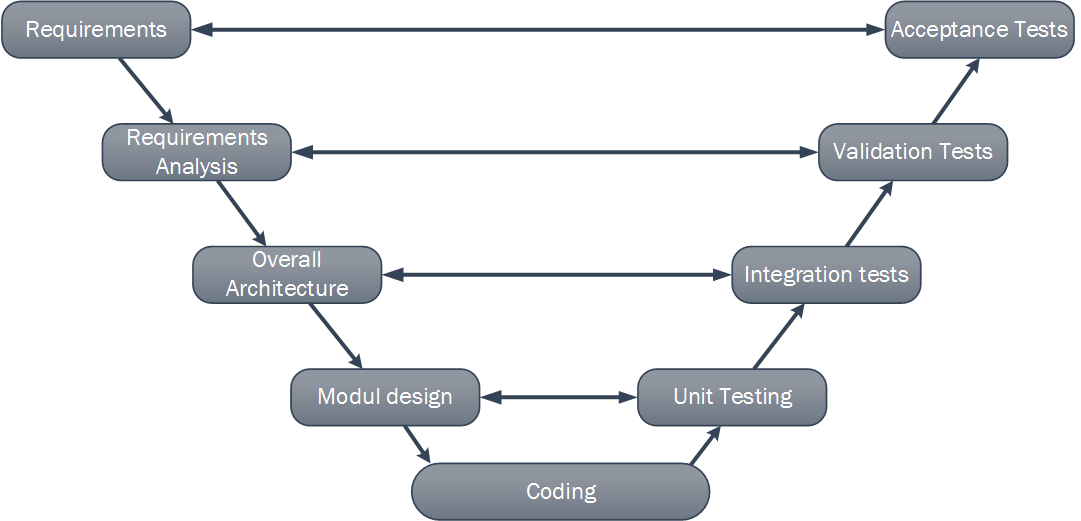
\includegraphics[width=1\textwidth]{resources/images/vmodel}
    \caption{V-model representation}\label{fig:contrib2:v}
\end{figure}
Since that the several steps of the V-model are sequentially passed through, each step should be completed before moving to the next one. Thus, the process starts by analyzing and collecting the requirements. Based on the collected requirements, the overall design system architecture is documented. Afterward, the implementation step starts by developing the core skeleton of the design previously documented and sequentially adding new functional units. Finally as illustrated in figure~\ref{fig:contrib2:v} there are several steps used to validate the process with various tests (e.g. Unit testing, component testing\ldots).

\section{Project Structure}

%But there are several programming language used for implementing the user interfaces within this work.

%As it was described in the chapter, the OpenMTC feature are aligned with the oneM2M specification. Therefore it implements a CSE at the Front-end gateway and a second CSE at the back-end server. Moreover it provides several method to communicate with non-M2M enabled devices through dedicated Inter-working proxy Entities. \par 

%This extension allows OpenMTC to create a pool of common data available in a specific environment and to share them between different OpenMTC applications, without requiring the information of the data type or content (units, meta data, context, etc.) in advance. Moreover, our implementation consist as well in enabling data access via SPARQL interface and oneM2M standard. \par 
%As outlined in the previous chapter, the goal of this thesis is to design and implement a semantic annotation extension for the OpenMTC Platform aiming to provide semantic interoperability for accessing resources and interpreting data from different stakeholders. \par 


%reference for the device and everything



\section{Conclusion}

\sidenote{Summary}
\todomid{write}

\sidenote{Takeaway 1}
\todomid{write}

\sidenote{Takeaway 2}
\todomid{write}

\sidenote{Takeaway 3}
\todomid{write}

\sidenote{Next chapter}
\todomid{write}
